%\documentclass[hyperref={pdfpagelabels=false},slidetop,9pt]{beamer}
\documentclass[slidetop,8pt]{beamer}
\usepackage[T1]{fontenc}
\usepackage[utf8]{inputenc}
\newcommand{\id}{71}
\newcommand{\nom}{Théorie des mécanismes}
\newcommand{\sequence}{04}
\newcommand{\nomsequence}{Liaisons entre les solides}
\newcommand{\num}{02}
\newcommand{\type}{KH}
\newcommand{\descrip}{Liaisons équivalentes, hyperstatisme, liaisons en série et en parallèle, théorie des graphes}
\newcommand{\competences}{B2-12: Proposer une modélisation des liaisons avec leurs caractéristiques géométriques. \\ &  B2-13: Proposer un modèle cinématique paramétré à partir d'un système réel, d'une maquette numérique ou d'u \\ &  B2-17: Simplifier un modèle de mécanisme. \\ &  B2-18: Modifier un modèle pour le rendre isostatique. \\ &  C1-04: Proposer une démarche permettant d'obtenir une loi entrée-sortie géométrique.  \\ &  C2-05: Caractériser le mouvement d'un repère par rapport à un autre repère. \\ &  C2-06: Déterminer les relations entre les grandeurs géométriques ou cinématiques. }
\newcommand{\nbcomp}{7}
\newcommand{\systemes}{}
\newcommand{\systemesnum}{}
\newcommand{\systemessansaccent}{}
\newcommand{\ilot}{2}
\newcommand{\ilotstr}{02}
\newcommand{\dossierilot}{\detokenize{Ilot_02 }}

\usepackage{etex}
\usepackage{tikz}
\usepackage[european]{circuitikz}
\usepackage{pgf}
\usepackage[all]{xy}
\usepackage{pgfpages}
\usepackage{graphbox}
\usepackage{pdfpages}
%\usepackage[adobe-utopia]{mathdesign}
\usepackage{ifthen}
\usepackage{cancel}
\usepackage{framed}
\usepackage{subfig}
\usepackage{tabularx}
\usepackage{setspace}
\usepackage{soul}
\usepackage{schemabloc}
\usepackage{eqnarray}
\usepackage[dot, phantomtext]{dashundergaps}
\usepackage{media9}
\usepackage{multimedia}
\usepackage{textcomp}
\usefonttheme[onlymath]{serif}

\author{Renaud Costadoat}
\institute{Lycée Dorian}

\usepackage{multido}
\usepackage{multirow}
\usepackage{multicol} % Portions de texte en colonnes
\usepackage{flafter}%floatants après la référence

\usepackage{color}
\usepackage{xcolor}
\usepackage{colortbl}

\usepackage[gen]{eurosym}
\usepackage{tikz}
%\usepackage{pstricks,pst-node,pst-tree,pst-solides3d}
\usepackage{lmodern}
\usepackage[francais]{babel}
\usepackage{pslatex}
\usetheme{renaud}
\usepackage{times}
\usepackage[frenchmath]{newtxsf} % for sans serif symbols
\renewcommand{\familydefault}{\sfdefault}
%\usepackage{amsfonts}
%\usepackage{amsmath}
%\usepackage{mathastext}
\usepackage{verbatim}
\usepackage{moreverb}
%\usetikzlibrary{arrows,shapes}
\usepackage{graphicx}
\usepackage{psfrag}
\usepackage{wrapfig}
\usepackage{etoolbox}

\definecolor{gris25}{gray}{0.75}
\definecolor{bleu}{RGB}{18,33,98}
\definecolor{bleuf}{RGB}{42,94,171}
\definecolor{bleuc}{RGB}{231,239,247}
\definecolor{rougef}{RGB}{185,18,27}
\definecolor{rougec}{RGB}{255,188,204}%255,230,231
\definecolor{vertf}{RGB}{103,126,82}
\definecolor{vertc}{RGB}{220,255,191}

\setlength\parindent{24pt}
\parskip 7.2pt
\parindent 8pt

\newenvironment{rem}[1][\hsize]%
{%
    \def\FrameCommand
   {%
\rotatebox{90}{\textit{\textsf{Remarque}}} 
       {\color{bleuf}\vrule width 3pt}%
       \hspace{0pt}%must no space.
       \fboxsep=\FrameSep\colorbox{bleuc}%
  }%
    \MakeFramed{\hsize#1\advance\hsize-\width\FrameRestore}%
}%
{\endMakeFramed}%


\newenvironment{savoir}[1][\hsize]%
{%
    \def\FrameCommand
    {%
\rotatebox{90}{\textit{\textsf{Savoir}}} 
        {\color{bleuf}\vrule width 3pt}%
        \hspace{0pt}%must no space.
        \fboxsep=\FrameSep\colorbox{bleuc}%
    }%
    \MakeFramed{\hsize#1\advance\hsize-\width\FrameRestore}%
}%
{\endMakeFramed}%

\newenvironment{prob}[1][\hsize]%
{%
    \def\FrameCommand%
    {%
\rotatebox{90}{\textit{\textsf{Problematique}}} 
        {\color{rougef}\vrule width 3pt}%
        \hspace{0pt}%must no space.
        \fboxsep=\FrameSep\colorbox{rougec}%
    }%
    \MakeFramed{\hsize#1\advance\hsize-\width\FrameRestore}%
}%
{\endMakeFramed}%

\newenvironment{obj}[1][\hsize]%
{%
    \def\FrameCommand%
    {%
\rotatebox{90}{\textit{\textsf{Objectif}}} 
        {\color{vertf}\vrule width 3pt}%
        \hspace{0pt}%must no space.
        \fboxsep=\FrameSep\colorbox{vertc}%
    }%
    \MakeFramed{\hsize#1\advance\hsize-\width\FrameRestore}%
}%
{\endMakeFramed}%

\newenvironment{defi}[1][\hsize]%
{%
    \def\FrameCommand%
    {%
\rotatebox{90}{\textit{\textsf{Definition}}} 
        {\color{bleuf}\vrule width 3pt}%
        \hspace{0pt}%must no space.
        \fboxsep=\FrameSep\colorbox{rougec}%
    }%
    \MakeFramed{\hsize#1\advance\hsize-\width\FrameRestore}%
}%
{\endMakeFramed}%


\newenvironment{hypo}[1][\hsize]%
{%
    \def\FrameCommand%
    {%
\rotatebox{90}{\textit{\textsf{Hypothèse\\}}} 
        {\color{bleuf}\vrule width 3pt}%
        \hspace{0pt}%must no space.
        \fboxsep=\FrameSep\colorbox{bleuc}%
    }%
    \MakeFramed{\hsize#1\advance\hsize-\width\FrameRestore}%
}%
{\endMakeFramed}%


\newenvironment{prop}[1][\hsize]%
{%
    \def\FrameCommand%
    {%
\rotatebox{90}{\textit{\textsf{Propriété}}} 
        {\color{bleuf}\vrule width 3pt}%
        \hspace{0pt}%must no space.
        \fboxsep=\FrameSep\colorbox{bleuc}%
    }%
    \MakeFramed{\hsize#1\advance\hsize-\width\FrameRestore}%
}%
{\endMakeFramed}%

\newenvironment{props}[1][\hsize]%
{%
    \def\FrameCommand%
    {%
\rotatebox{90}{\textit{\textsf{Propriétés}}} 
        {\color{bleuf}\vrule width 3pt}%
        \hspace{0pt}%must no space.
        \fboxsep=\FrameSep\colorbox{bleuc}%
    }%
    \MakeFramed{\hsize#1\advance\hsize-\width\FrameRestore}%
}%
{\endMakeFramed}%

\newenvironment{exemple}[1][\hsize]%
{%
    \def\FrameCommand%
    {%
\rotatebox{90}{\textit{\textsf{Exemple}}} 
        {\color{vertf}\vrule width 3pt}%
        \hspace{0pt}%must no space.
        \fboxsep=\FrameSep\colorbox{vertc}%
    }%
    \MakeFramed{\hsize#1\advance\hsize-\width\FrameRestore}%
}%
{\endMakeFramed}%

\newenvironment{resultat}[1][\hsize]%
{%
    \def\FrameCommand%
    {%
\rotatebox{90}{\textit{\textsf{Résultat}}} 
        {\color{rougef}\vrule width 3pt}%
%        {\color{bleuf}\vrule width 3pt}%
        \hspace{0pt}%must no space.
        \fboxsep=\FrameSep\colorbox{rougec}%
    }%
    \MakeFramed{\hsize#1\advance\hsize-\width\FrameRestore}%
}%
{\endMakeFramed}%

\newenvironment{methode}[1][\hsize]%
{%
    \def\FrameCommand%
    {%
\rotatebox{90}{\textit{\textsf{Méthode\\}}} 
        {\color{rougef}\vrule width 3pt}%
        \hspace{0pt}%must no space.
        \fboxsep=\FrameSep\colorbox{rougec}%
    }%
    \MakeFramed{\hsize#1\advance\hsize-\width\FrameRestore}%
}%
{\endMakeFramed}%

\newenvironment{theo}[1][\hsize]%
{%
    \def\FrameCommand%
    {%
\rotatebox{90}{\textit{\textsf{Théorème\\}}} 
        {\color{rougef}\vrule width 3pt}%
        \hspace{0pt}%must no space.
        \fboxsep=\FrameSep\colorbox{rougec}%
    }%
    \MakeFramed{\hsize#1\advance\hsize-\width\FrameRestore}%
}%
{\endMakeFramed}%

\newenvironment{warn}[1][\hsize]%
{%
    \def\FrameCommand%
    {%
\rotatebox{90}{\textit{\textsf{Attention\\}}} 
        {\color{rougef}\vrule width 3pt}%
        \hspace{0pt}%must no space.
        \fboxsep=\FrameSep\colorbox{rougec}%
    }%
    \MakeFramed{\hsize#1\advance\hsize-\width\FrameRestore}%
}%
{\endMakeFramed}%

% \usepackage{pstricks}
%\usepackage{minitoc}
% \setcounter{minitocdepth}{4}

\setcounter{tocdepth}{2}

% \mtcselectlanguage{french} 

%\usepackage{draftcopy}% "Brouillon"
% \usepackage{floatflt}
\usepackage{psfrag}
%\usepackage{listings} % Permet d'insérer du code de programmation
\renewcommand{\baselinestretch}{1.2}

% Changer la num�rotation des figures :
% ------------------------------------
% \makeatletter
% \renewcommand{\thefigure}{\ifnum \c@section>\z@ \thesection.\fi
%  \@arabic\c@figure}
% \@addtoreset{figure}{section}
% \makeatother
 


%%%%%%%%%%%%
% Définition des vecteurs %
%%%%%%%%%%%%
 \newcommand{\vect}[1]{\overrightarrow{#1}}

%%%%%%%%%%%%
% Définition des torseusr %
%%%%%%%%%%%%

 \newcommand{\torseur}[1]{%
\left\{{#1}\right\}
}

\newcommand{\torseurcin}[3]{%
\left\{\mathcal{#1} \left(#2/#3 \right) \right\}
}

\newcommand{\torseurstat}[3]{%
\left\{\mathcal{#1} \left(#2\rightarrow #3 \right) \right\}
}

 \newcommand{\torseurc}[8]{%
%\left\{#1 \right\}=
\left\{
{#1}
\right\}
 = 
\left\{%
\begin{array}{cc}%
{#2} & {#5}\\%
{#3} & {#6}\\%
{#4} & {#7}\\%
\end{array}%
\right\}_{#8}%
}

 \newcommand{\torseurcol}[7]{
\left\{%
\begin{array}{cc}%
{#1} & {#4}\\%
{#2} & {#5}\\%
{#3} & {#6}\\%
\end{array}%
\right\}_{#7}%
}

 \newcommand{\torseurl}[3]{%
%\left\{\mathcal{#1}\right\}_{#2}=%
\left\{%
\begin{array}{l}%
{#1} \\%
{#2} %
\end{array}%
\right\}_{#3}%
}

 \newcommand{\vectv}[3]{%
\vect{V\left( {#1} \in {#2}/{#3}\right)}
}


\newcommand{\vectf}[2]{%
\vect{R\left( {#1} \rightarrow {#2}\right)}
}

\newcommand{\vectm}[3]{%
\vect{\mathcal{M}\left( {#1}, {#2} \rightarrow {#3}\right)}
}


 \newcommand{\vectg}[3]{%
\vect{\Gamma \left( {#1} \in {#2}/{#3}\right)}
}

 \newcommand{\vecto}[2]{%
\vect{\Omega\left( {#1}/{#2}\right)}
}

\newcommand{\reponse}[1][4]
{
\multido{}{#1}
{
\begin{center}
\makebox[0.9\linewidth]{\dotfill} \end{center}
}}


% }$$\left\{\mathcal{#1} \right\}_{#2} =%
% \left\{%
% \begin{array}{c}%
%  #3 \\%
%  #4 %
% \end{array}%
% \right\}_{#5}}


%  ------------------------------------------
% | Modification du formatage des sections : | 
%  ------------------------------------------

% Grands titres :
% ---------------

\newcommand{\titre}[1]{%
\begin{center}
      \bigskip
      \rule{\textwidth}{1pt}
      \par\vspace{0.1cm}
      
      \textbf{\large #1}
      \par\rule{\textwidth}{1pt}
    \end{center}
    \bigskip
  }

% Supprime le numéro du chapitre dans la numérotation des sections:
% -----------------------------------------------------------------
\makeatletter
\renewcommand{\thesection}{\@arabic\c@section}
\makeatother


% \titleformat{\chapter}[display]
% {\normalfont\Large\filcenter}
% {}
% {1pc}
% {\titlerule[1pt]
%   \vspace{1pc}%
%   \Huge}[\vspace{1ex}%
% \titlerule]


%%%% Chapitres Comme PY Pechard %%%%%%%%%
% numéro du chapitre
\DeclareFixedFont{\chapnumfont}{OT1}{phv}{b}{n}{80pt}
% pour le mot " Chapitre "
\DeclareFixedFont{\chapchapfont}{OT1}{phv}{m}{it}{40pt}
% pour le titre
\DeclareFixedFont{\chaptitfont}{T1}{phv}{b}{n}{25pt}

\definecolor{gris}{gray}{0.75}
\setbeamertemplate{section in toc}[sections numbered]

\newlength{\RoundedBoxWidth}
\newsavebox{\GrayRoundedBox}
\newenvironment{GrayBox}[1][\dimexpr\textwidth-4.5ex]%
   {\setlength{\RoundedBoxWidth}{\dimexpr#1}
    \begin{lrbox}{\GrayRoundedBox}
       \begin{minipage}{\RoundedBoxWidth}}%
   {   \end{minipage}
    \end{lrbox}
    \begin{center}
    \begin{tikzpicture}%
       \draw node[draw=bleuf,fill=bleuc,rounded corners,%
             inner sep=2ex,text width=\RoundedBoxWidth]%
             {\usebox{\GrayRoundedBox}};
    \end{tikzpicture}
    \end{center}}
    
\ifdef{\prive}{\pgfpagesuselayout{2 on 1}[a4paper,border shrink=0mm]}
\ifdef{\prive}{\setbeamertemplate{navigation symbols}{}}
\setbeamertemplate{itemize item}[ball]
%\setbeamertemplate{blocks}[rounded]%[shadow=true]
\setbeamercolor{block title}{fg=white,bg=grisf}        % titre block normal 
\setbeamercolor{block body}{fg=grisf,bg=grisc!50}      % corps block normal
\setbeamercolor{block body alerted}{fg=white,bg=warning}   % idem pour un block alerte

\title{\nom}
\date{S\sequence \ - \type\num}

\begin{document}
\shorthandoff{:!}
\bibliographystyle{abbrvnat-fr}

\usebackgroundtemplate%
{%
    \centering
\includegraphics[width=\paperwidth]{/home/renaud/Documents/Renaud/GitHub/Sciences-Ingenieur/img/fond2}%
}

{
\setbeamertemplate{navigation symbols}{}
\setbeamertemplate{headline}[pagetitre]
\setbeamertemplate{footline}[pagetitre]
\usebackgroundtemplate{\centering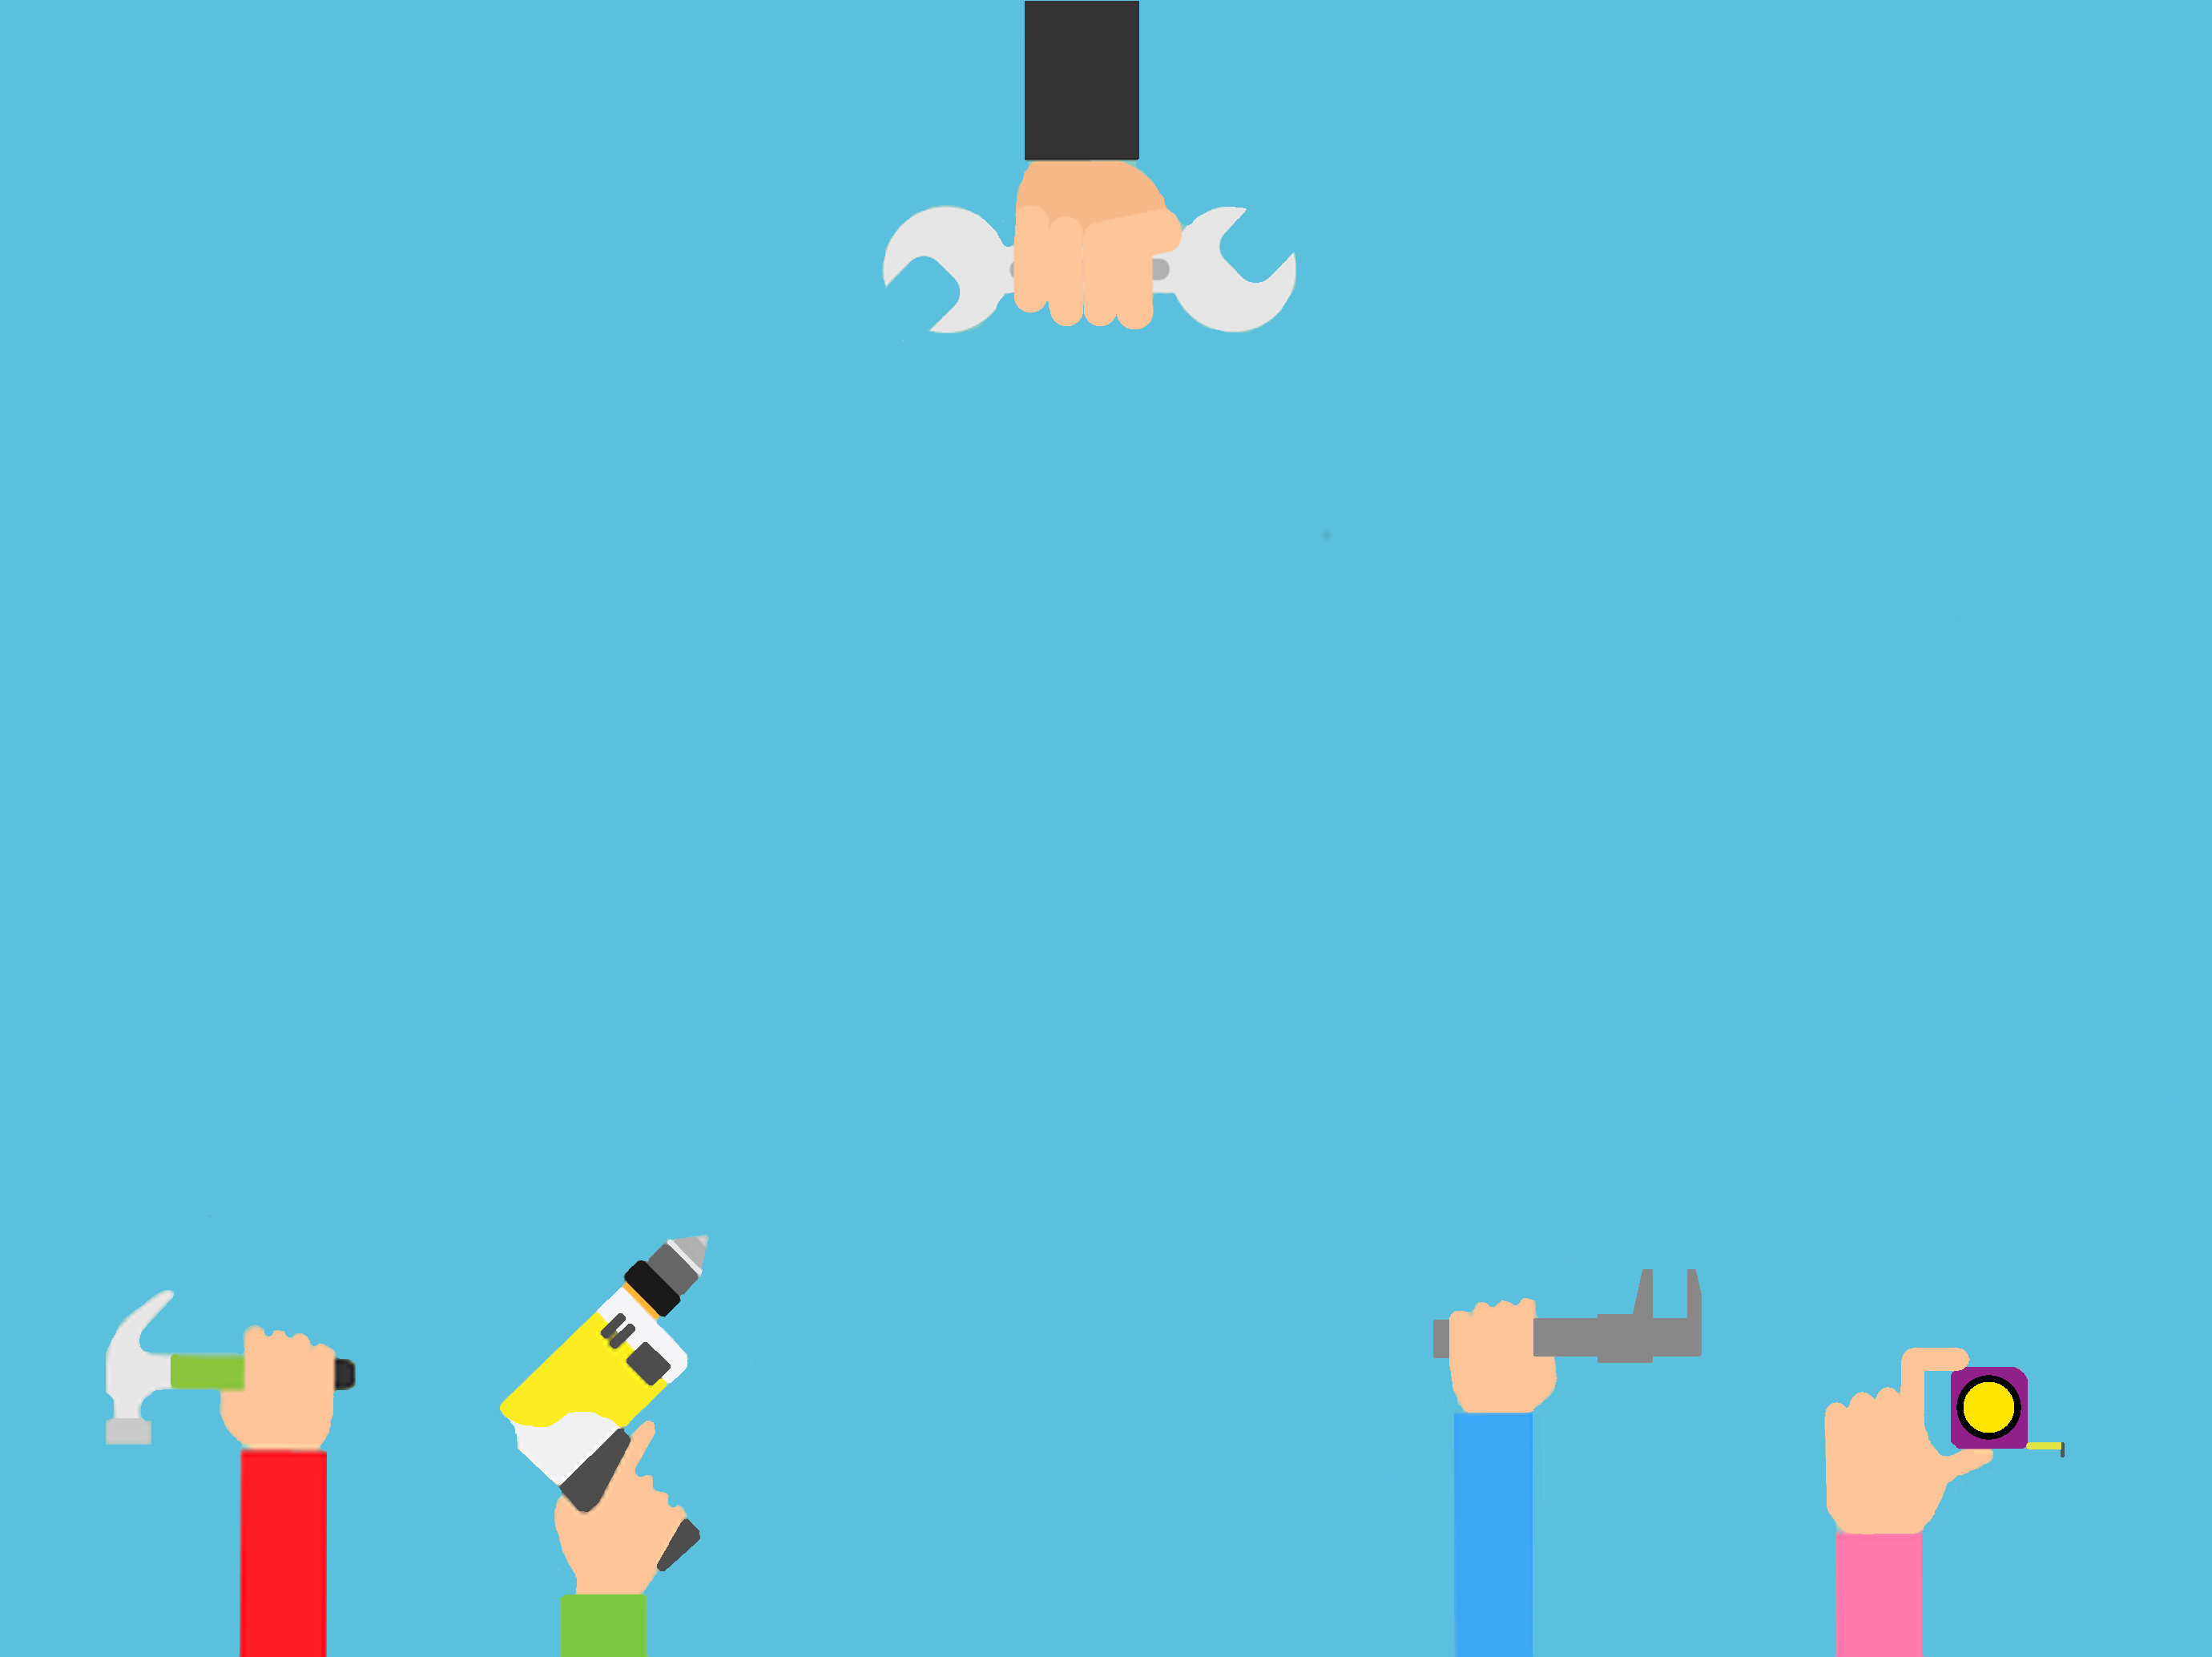
\includegraphics[width=\paperwidth]{/home/renaud/Documents/Renaud/GitHub/Sciences-Ingenieur/img/fond}}
\frame{\titlepage}
}



\section{Introduction}

\ifdef{\prive}{}{\begin{frame}
\frametitle{Table des matières}
\tableofcontents[currentsection]
\end{frame}}

{\frame{
\frametitle{Les Sciences de l'Ingénieur}

L'objectif des \textbf{sciences de l'ingénieur} est de donner accès aux étudiants à des \textbf{méthodes raisonnement} ainsi qu'à une \textbf{culture technologique} leur permettant de faire face à des \textbf{problématiques} liées à des \textbf{systèmes complexes}.

Le système est le point central de l'étude. Il peut être 
\begin{itemize}
 \item \textbf{multi-physique}: lier de l'énergie mécanique, électrique, thermique, chimique,...
 \item\textbf{multi-échelle}: lier des phénomènes à des échelles très différentes.
\end{itemize}

\begin{figure}
\begin{minipage}{0.60\linewidth}
\begin{defi}
\textit{\textsf{Système} \\}
Un système est un ensemble d'éléments qui interagissent entre eux. Ces interactions sont régies par des principes ou règles.
\end{defi}
\end{minipage}
\hfill
\begin{minipage}{0.30\linewidth}
\centering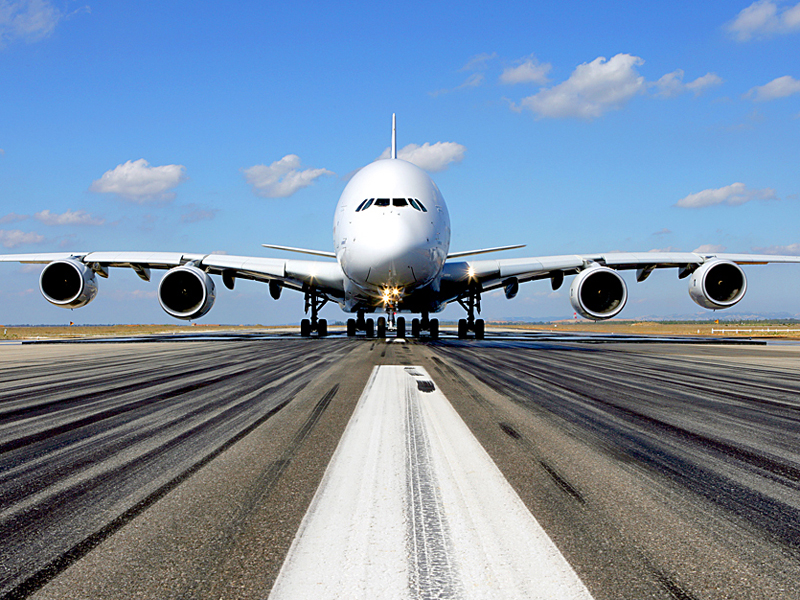
\includegraphics[width=0.8\linewidth]{img/fig5}
\caption{Avion Airbus\textregistered}
\end{minipage}
\end{figure}

}}

{\frame{
\frametitle{L'ingénierie système}

\begin{figure}[!h]
 \begin{minipage}{0.72\linewidth}
La \textbf{complexité} d'un système tient au fait que les relations qui lient ses composants soient \textit{multiples}, \textit{interdépendantes} et \textit{bouclées}. Le comportement global n'est alors pas directement prévisible à partir des comportements élémentaires des composants.
 \end{minipage}
 \hfill
 \begin{minipage}{0.25\linewidth}
 \centering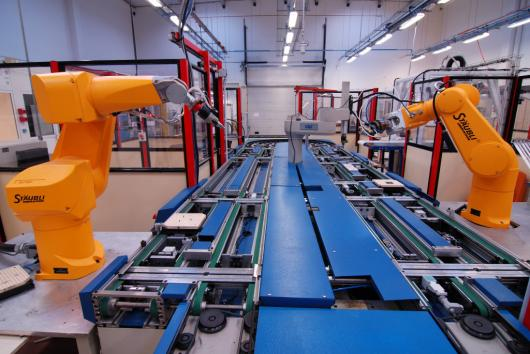
\includegraphics[width=0.8\linewidth]{img/transfert.jpg}
 \end{minipage}
\end{figure}

\begin{defi}
L'\textbf{ingénierie système} est une approche scientifique interdisciplinaire qui permet d'appréhender la conception de systèmes complexes. Elle passe en partie par l'analyse de solutions antérieures afin de répondre aux problématiques actuelles.
\end{defi}

\vspace{-0.3cm}

Processus de \textbf{conception} d'un produit complexe:
\vspace{-0.2cm}
\begin{itemize}
 \item \textbf{analyse de l'existant} (appropriation).
 \begin{enumerate}
  \item \textbf{Analyse} du système: Pourquoi le système a-t-il été conçu de cette façon ?
  \item Proposition de \textbf{reconception/évolution}: Comment le système peut-il évoluer ?
 \end{enumerate}
 \item \textbf{innovation} (nouvelles solutions),
 \begin{enumerate}
  \item Capture du \textbf{besoin}: Quel est le souhait du client ?
  \item Recherche de \textbf{solutions techniques}: Quelle solution va le satisfaire au mieux ?
 \end{enumerate}
\end{itemize}

}}

\section{Du besoin aux exigences}

\ifdef{\prive}{}{
\begin{frame}
\frametitle{Table des matières}
\tableofcontents[currentsection]
\end{frame}}
 
{\frame{
\frametitle{Analyser un système}

\begin{obj}
Découvrir les \textbf{outils} et des \textbf{méthodes} structurants liés à l'\textbf{analyse des systèmes} en suivant le processus d'une \textbf{conception}.

En travaillant dans ce sens, il est possible de se \textit{mettre à la place} du concepteur en effectuant l'analyse d'un système \textbf{existant}.
\end{obj}

\begin{figure}
\centering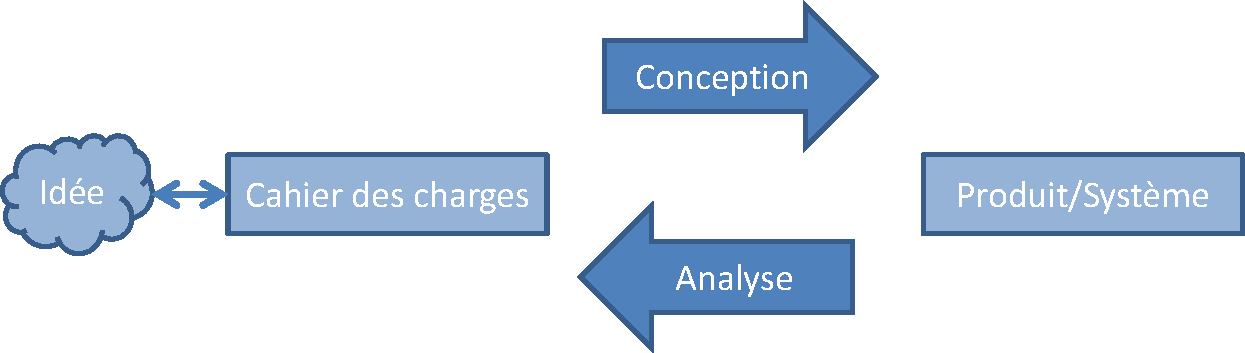
\includegraphics[width=0.6\linewidth]{img/fig1}
\caption{Processus de \textbf{Conception/Analyse}}
\end{figure}
}}

{\frame{
\frametitle{Concevoir un système}

\begin{figure}
 \begin{minipage}{0.37\linewidth}
L'\textbf{entreprise}, au sein de laquelle travaille le concepteur, part du \textbf{besoin du client} et suit des \textbf{axes de contraintes} qui limitent la liberté du concepteur:
\begin{itemize}
 \item La compétitivité
 \item La productivité
 \item La qualité
 \item L'interchangeabilité
\end{itemize}

Le travail à effectuer est réparti sur 3 principales entités :
\begin{itemize}
 \item \textbf{Bureau d'etude},
 \item \textbf{Bureau des méthodes}
 \item \textbf{Production} 
\end{itemize}
 \end{minipage}
\hfill
 \begin{minipage}{0.6\linewidth}
 \centering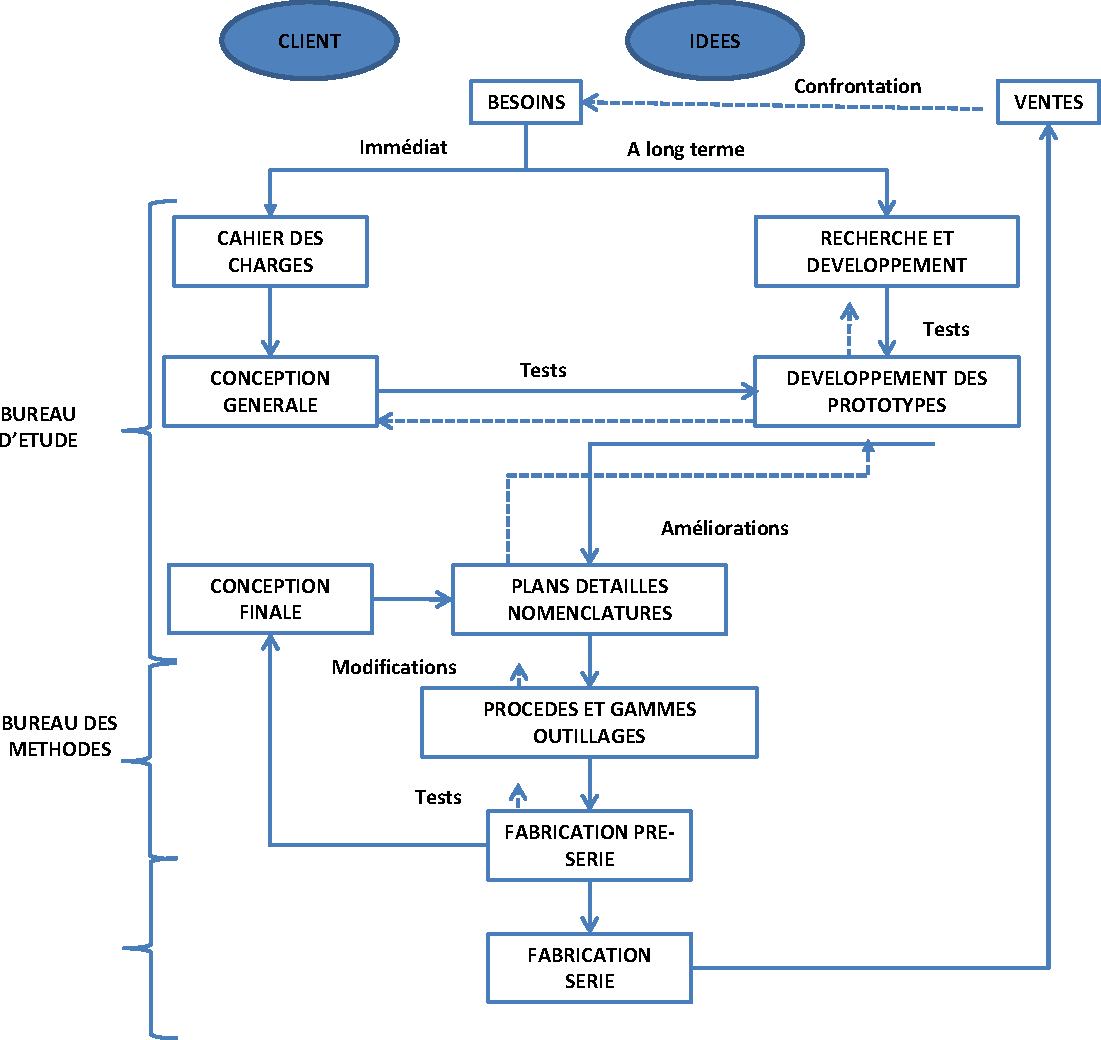
\includegraphics[width=1\linewidth]{img/fig6}
 \caption{Les étapes de la conception}
 \end{minipage}
\end{figure}
}}

{\frame{
\frametitle{La Capture du besoin}

La première étape de la relation client fournisseur est généralement la \textbf{Capture du Besoin}. Elle consiste à sonder le \textbf{client/utilisateur} afin de définir le \textbf{Besoin}.

\vspace{0.5cm}

\begin{minipage}{0.7\linewidth}
\begin{defi}
 \textit{\textsf{Besoin X50-150}} \\
Le besoin est une nécessité ou un désir éprouvé par \textbf{l'utilisateur}. Ce besoin peut être \textbf{exprimé} par l'utilisateur ou \textbf{latent} (ou potentiel). C'est la fonction de la mercatique de définir un modèle d'utilisateur-client en terme de besoin.
\end{defi}

\end{minipage}
\hfill
\begin{minipage}{0.25\linewidth}
 \centering
\includegraphics[width=0.8\linewidth]{img/fig7}
\end{minipage}

\vspace{0.5cm}

Ainsi, le besoin peut être défini comme l'ensemble de ce qui apparaît être nécessaire. Le concepteur doit, si possible, intégrer toutes les demandes du client avant de commencer sa conception. Un oubli peut parfois être très problématique.
}}


{\frame{
\frametitle{Le cycle de vie}

L'une des méthodes permettant d'obtenir de bons résultats en terme de cahier des charges consiste à \textbf{décomposer} le \textbf{cycle de vie} du produit en \textbf{phases de vie}.

\begin{defi}
\textit{\textsf{Analyse du Cycle de vie  X50-151}} \\
L'analyse du cycle de vie (ACV) est une activité issue du développement durable qui permet d'évaluer les impacts environnementaux d'un produit, d'un service, d'une entreprise ou d'un procédé.
\end{defi}

\begin{figure}[!h]
\begin{minipage}{0.2\linewidth}
 \centering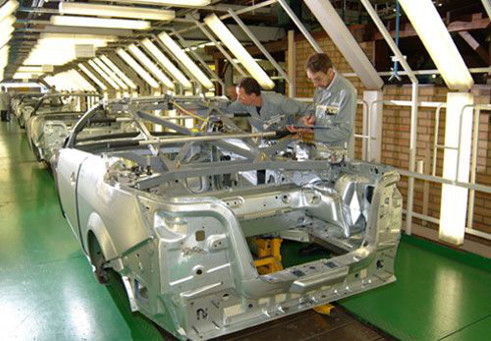
\includegraphics[height=1.5cm]{img/fig8}
\end{minipage}
\hfill
\begin{minipage}{0.23\linewidth}
 \centering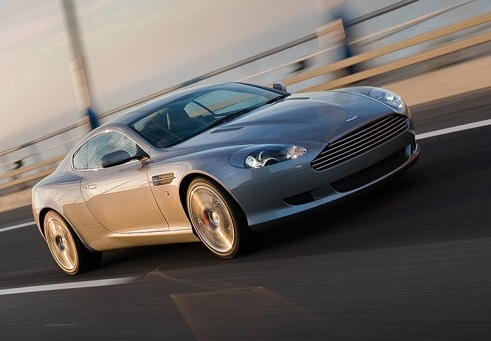
\includegraphics[height=1.5cm]{img/fig9}
\end{minipage}
\hfill
\begin{minipage}{0.23\linewidth}
 \centering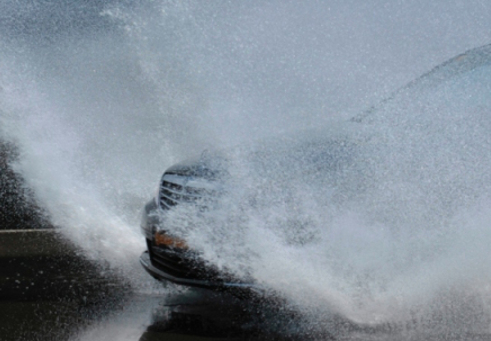
\includegraphics[height=1.5cm]{img/fig10}
\end{minipage}
\hfill
\begin{minipage}{0.23\linewidth}
 \centering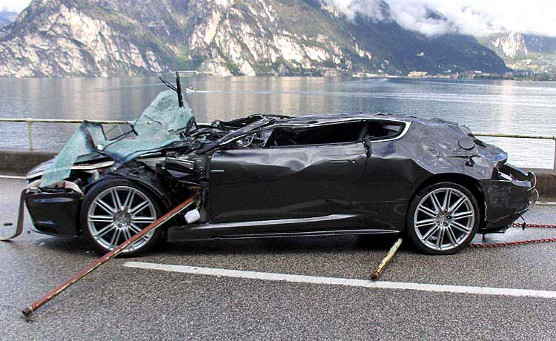
\includegraphics[height=1.5cm]{img/fig11}
\end{minipage}

\caption{Phases de vie d'une Aston Martin \textregistered}
\end{figure}
}}

{\frame{
\frametitle{Les phases de vie}

Le cycle de vie d'un produit se décompose en \textbf{phases de vie}, les principales sont les suivantes:

\begin{center}
 \begin{tabular}{|l|l|l|l|}
 \hline
 fabrication & transport & stockage & vente \\
 \hline
 utilisation & maintenance & recyclage & ... \\
 \hline
 \end{tabular}
\end{center}

Les exigences liées au produit varient souvent au cours du temps.

\begin{exemple}
  \begin{minipage}{0.65\linewidth}
 Un célèbre constructeur automobile ayant mal étudié la phase de vie \og transport \fg lors de la conception d'un de ses modèles, n'avait pas imaginé que ses véhicules puissent rouler à la vitesse de $100km.h^{-1}$ en marche arrière. Ainsi, l'ensemble des véhicules disposés de dos au déplacement du train ont vu leur plage arrière détrempée lors d'un jour pluvieux de transport.
 \end{minipage}
 \hfill
 \begin{minipage}{0.3\linewidth}
   \centering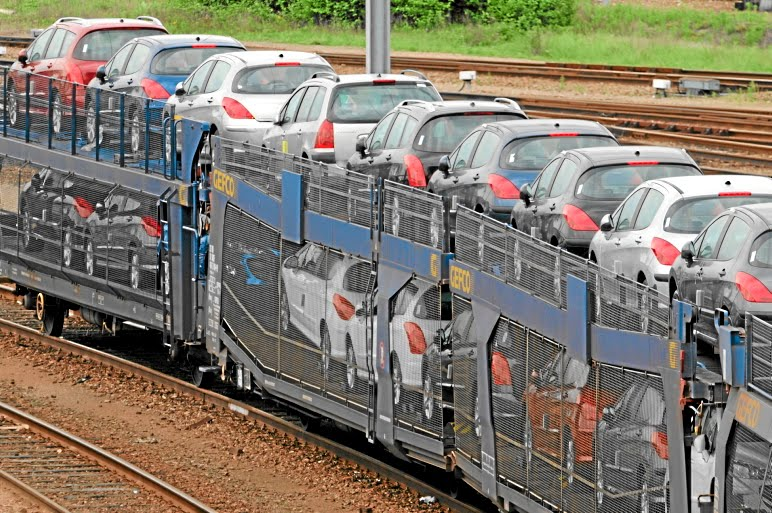
\includegraphics[width=\linewidth]{img/fret_auto.jpg}
 \end{minipage}
\end{exemple}

}}

{\frame{
\frametitle{Exemple du destructeur d'aiguille}

\begin{figure}[!h]
 \begin{minipage}{0.65\linewidth}
Un chirurgien dentiste a parfois besoin d'effectuer une anesthésie locale sur un patient afin d'effectuer un soin douloureux. Pour faire une anesthésie locale il utilise une seringue qui contient le produit anesthésiant.
 \end{minipage}
 \hfill
 \begin{minipage}{0.3\linewidth}
  \centering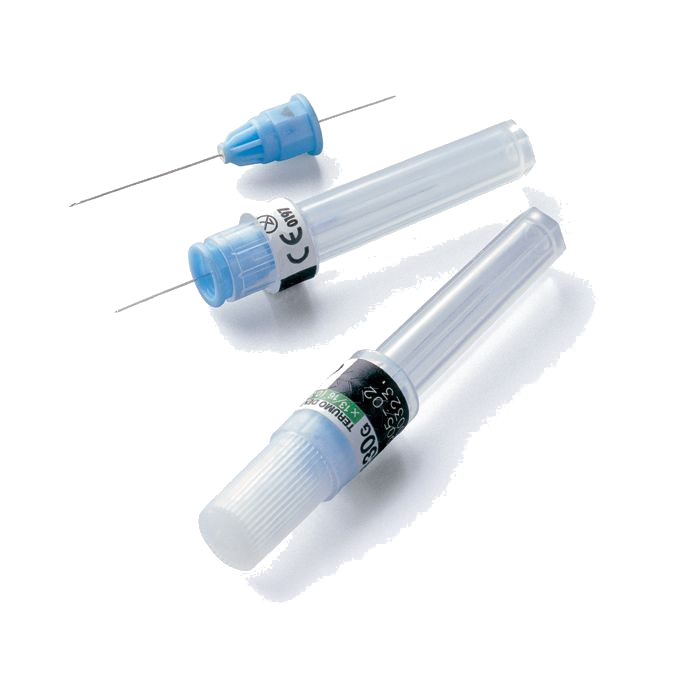
\includegraphics[width=0.9\linewidth]{img/aiguille}
 \end{minipage}
\end{figure}

\begin{figure}[!h]
 \begin{minipage}{0.3\linewidth}
   \centering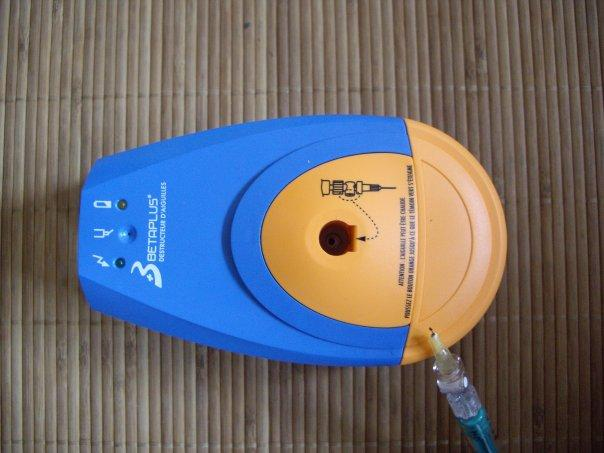
\includegraphics[width=0.9\linewidth]{img/destructeur}
 \end{minipage}
 \hfill
 \begin{minipage}{0.65\linewidth}
Le destructeur d'aiguille permet aux chirurgiens dentistes de détruire les aiguilles usagées sans risque de contamination. Il est entièrement automatisé afin que le dentiste n'ait pas à le manipuler alors que ces gants sont contaminés.
 \end{minipage}
\end{figure}

}}

{\frame{
\frametitle{Le cahier des charges}

Le besoin va être exprimé dans un \textbf{cahier des charges} qui servira de \textbf{contrat} entre le client et le concepteur.

\begin{defi}

\textit{\textsf{Le Cahier Des Charges Fonctionnel (C.D.C.F.) X50-151}}\\
Il s'agit d'un document par lequel le demandeur exprime son besoin au travers d'\textbf{exigences}.\\
\end{defi}

Pour chacune de ces exigences sont définis des \textbf{critères} d'appréciation et leurs \textbf{niveaux}. A chacun de ces niveaux est assortie une \textbf{flexibilité}.

\begin{figure}[!h]
 \begin{minipage}{0.65\linewidth}
\begin{defi}
Exigence:NF EN ISO 9000 \\
Besoin formulé, habituellement implicite ou imposé.
\end{defi}

 Il pourra être exprimé sous la forme d'un \textbf{Diagramme SysMl des Exigences}.
 \end{minipage}
 \hfill
 \begin{minipage}{0.33\linewidth}
 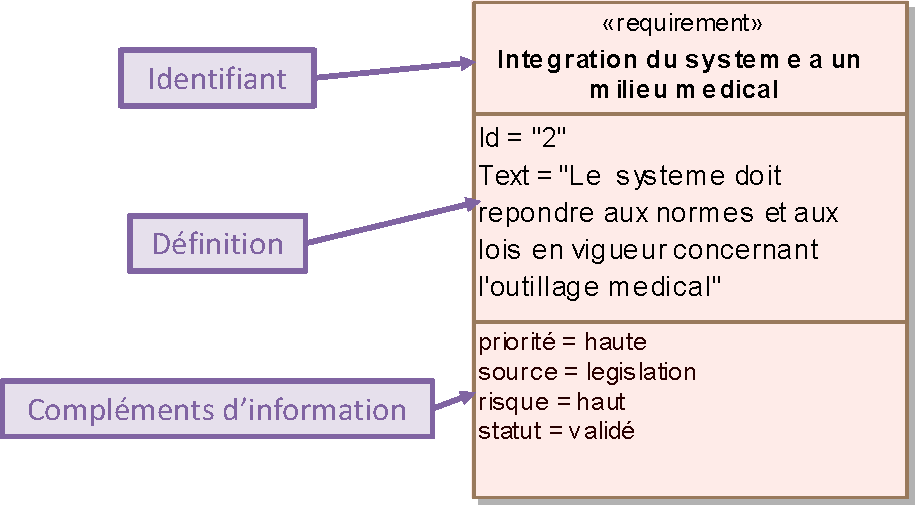
\includegraphics[width=\linewidth]{img/Diagramme_exigences_1}
 \caption{Diagramme d'Exigences}
 \end{minipage}
\end{figure}

}}

{\frame{
\frametitle{Les exigences}

\begin{figure}[!h]
\begin{minipage}{0.63\linewidth}
 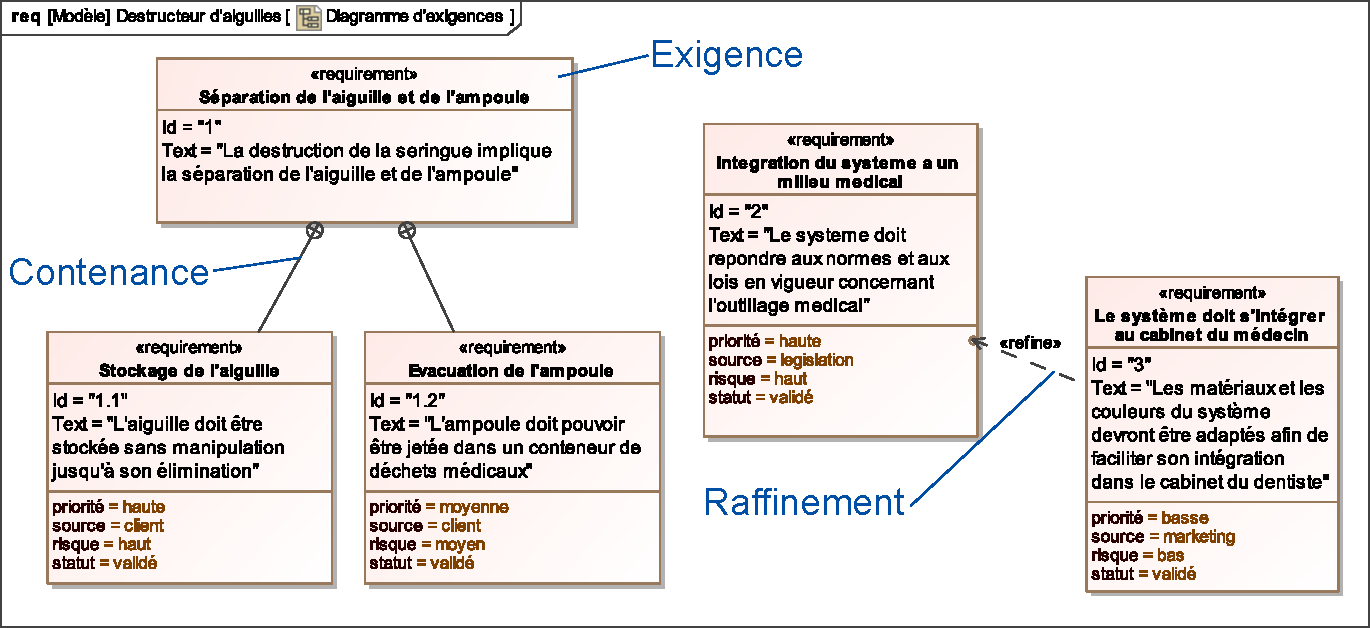
\includegraphics[width=\linewidth]{img/Diagramme_exigences}
 \caption{Diagramme d'Exigences}
\end{minipage}
 \hfill
\begin{minipage}{0.35\linewidth}
Ce diagramme est utilisé afin de décrire l'ensemble des \textbf{exigences} imposées à un système.


Les sources de ces exigences peuvent être multiples et être:
\begin{itemize}
 \item fonctionnelles (client),
 \item économiques,
 \item environnementales,
 \item techniques,...
\end{itemize}
\end{minipage}
\end{figure}

De par sa fonction de \og moelle épinière \fg, il est consulté à tout moment de l'étude. Ainsi, il doit être utilisé afin:
\begin{itemize}
 \item de \textbf{vérifier} que la construction de la solution reste en accord avec les C.D.C.F., 
 \item de \textbf{constater} les impacts sur le système de modification de la solution technique.
\end{itemize}
}}

{\frame{
\frametitle{Les exigences, et après...}


\begin{savoir}

Vous devez être capables de déterminer quelles exigences ont été à l'origine de la conception d'un produit.

\begin{itemize}
 \item Quelles sont les phases de vie du système ?
 \item A qui est-il destiné ?
\end{itemize}
\end{savoir}

\begin{prob}

Un système est souvent intégré dans un plus grand ensemble. 
\begin{itemize}
 \item \textit{Problème: Quelle est la part de ces services à attribuer au système étudié?}
 \item \textbf{Perspectives}: Déterminer à quelles attentes spécifiques répond un système: quelles sont ses frontières (physiques et fonctionnelles)
\end{itemize}
\end{prob}
}}

\section{Les frontières du système}

\ifdef{\prive}{}{
\begin{frame}
\frametitle{Table des matières}
\tableofcontents[currentsection]
\end{frame}}

{\frame{
\frametitle{Les frontières du système}

L'étude d'un système commence par son \textbf{isolement} de son \textbf{environnement}, il faut pour cela définir ses \textbf{limites} par rapport à cet environnement. Elles constituent sa \textbf{frontière d'isolement} et peuvent être \textit{physiques} ou \textit{fonctionnelles}.

Les éléments qui constituent l'\textbf{environnement} d'un système définissent le \textbf{contexte} de l'analyse.

\begin{exemple}
\begin{minipage}{0.65\linewidth}
Une prise électrique permet de connecter un appareil (grille pain, micro-onde, téléphone,...) au réseau électrique. Elle est donc indispensable au fonctionnement du système. Pourtant, il est évident qu'elle ne fait pas \og partie \fg du système.
\end{minipage}
\hfill
\begin{minipage}{0.3\linewidth}
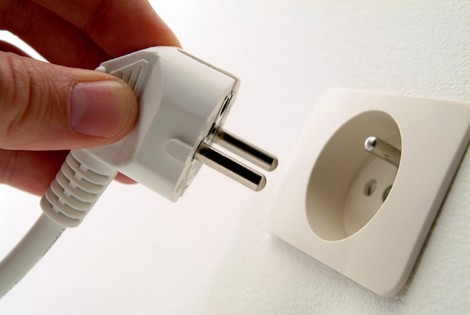
\includegraphics[width=0.8\linewidth]{img/prise.jpg}
\end{minipage}
\end{exemple}

}}

{\frame{
\frametitle{Le contexte}

\begin{figure}[!h]
\begin{minipage}{0.4\linewidth}
 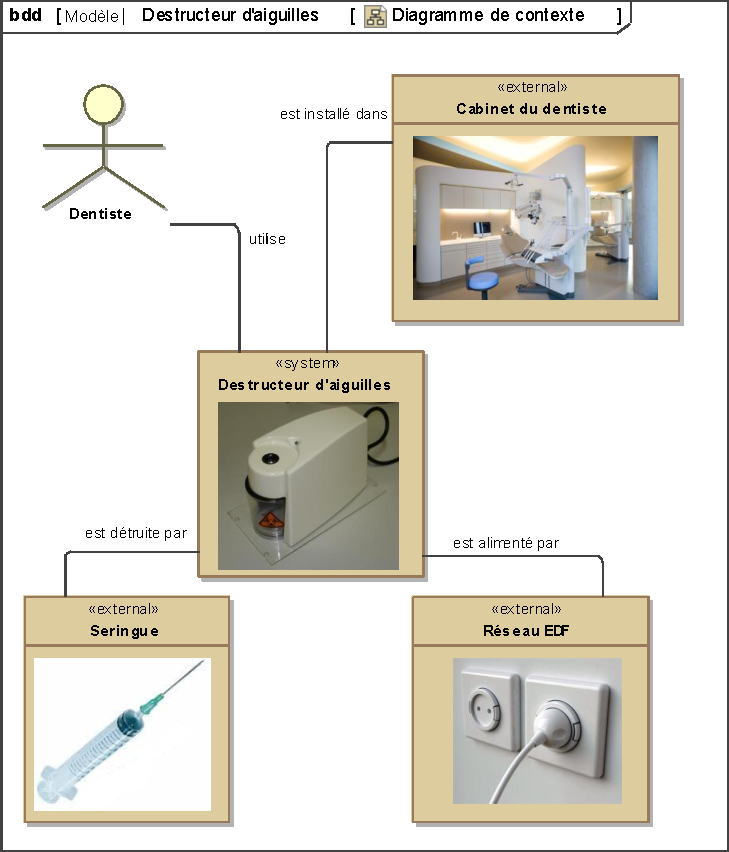
\includegraphics[width=\linewidth]{img/Diagramme_contexte}
 \caption{Diagramme de Contexte}
\end{minipage}
 \hfill
\begin{minipage}{0.58\linewidth}

Ce diagramme présente les \textbf{éléments} en \textbf{interaction} avec le système.

Certains groupes d'éléments se retrouvent de manière récurrente dans les diagrammes de contexte:
\begin{itemize}
 \item personnes (utilisateur, technicien),
 \item énergies (électricité, essence,...),
 \item environnement (air, eau,...),
 \item communications (internet, intranet),...
\end{itemize}

\begin{defi}
Une interaction est l'action ou l'influence réciproque qui peut s'établir entre deux objets ou plus.
\end{defi}
\end{minipage}
\end{figure}
}}

{\frame{
\frametitle{Quels services rend le système ?}

Le système existe pour offrir des \textbf{fonctionnalités}, elles constituent sa \textit{raison d'être}.

\begin{defi}
Une fonctionnalité peut être vue comme un \textbf{cas d'utilisation}. C'est un service rendu en \textbf{autonomie} par le système et dont le résultat est \textbf{visible} par l'acteur.

Un acteur est un élément externe qui interagit avec le système. Il peut être humain (utilisateur,...) ou non-humain (système-tier,...).

Une interactions correspond à l'action ou à l'influence réciproque entre des éléments.
\end{defi}

\begin{exemple}
\begin{minipage}{0.65\linewidth}
Un sabre laser fait de la lumière, mais pas seulement. Si une de ses fonctionnalités est oubliée dans le cahier des charges, il est possible qu'il soit remplacé par un produit qui ne conviendra pas.
\end{minipage}
 \hfill
\begin{minipage}{0.3\linewidth}
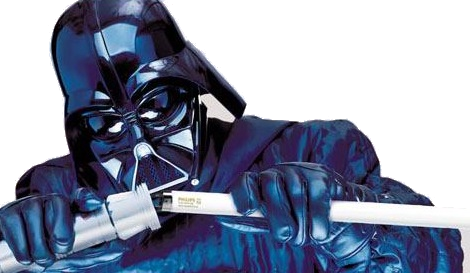
\includegraphics[width=\linewidth]{img/dark_neon}
\end{minipage}
\end{exemple}
}}

{\frame{
\frametitle{Les Services Attendus du système}

L'acteur est un élément externe privilégié car c'est lui qui va constater du service rendu par le système.

\begin{figure}[!h]
\begin{minipage}{0.7\linewidth}
L'\textbf{acteur} (celui qui va utiliser le système) sera en \textbf{interaction} avec celui-ci.

Il constatera la réponse du système, c'est pourquoi le concepteur va utiliser son point de vue afin de déterminer les \textbf{Services Attendus du système}.

\begin{defi}
 \textit{\textsf{Acteur - Services attendus du système - Interaction}}
 
Un acteur est un \textbf{élément externe} (humain ou non) qui \textbf{interagit} avec le système.

Un système doit proposer des \textbf{services attendus} afin de \textbf{satisfaire} le besoin de l'acteur.

Une \textbf{interaction} est l'action ou l'influence \textbf{réciproque} qui s'établit entre des éléments.
\end{defi}

\end{minipage}
\hfill
\begin{minipage}{0.25\linewidth}
 \centering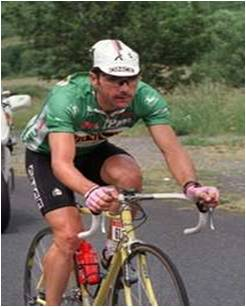
\includegraphics[width=0.6\linewidth]{img/fig14}
 \caption{Acteur}
 
 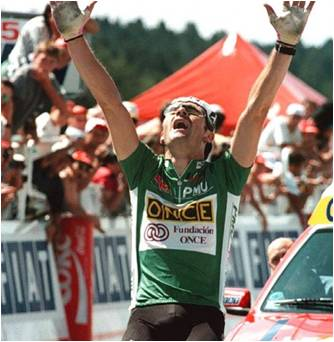
\includegraphics[width=0.6\linewidth]{img/fig15}
 \caption{Acteur \textbf{satisfait}}
\end{minipage}
\end{figure}

}}

{\frame{
\frametitle{Les cas d'utilisation}

\begin{figure}[!h]
\begin{minipage}{0.5\linewidth}
 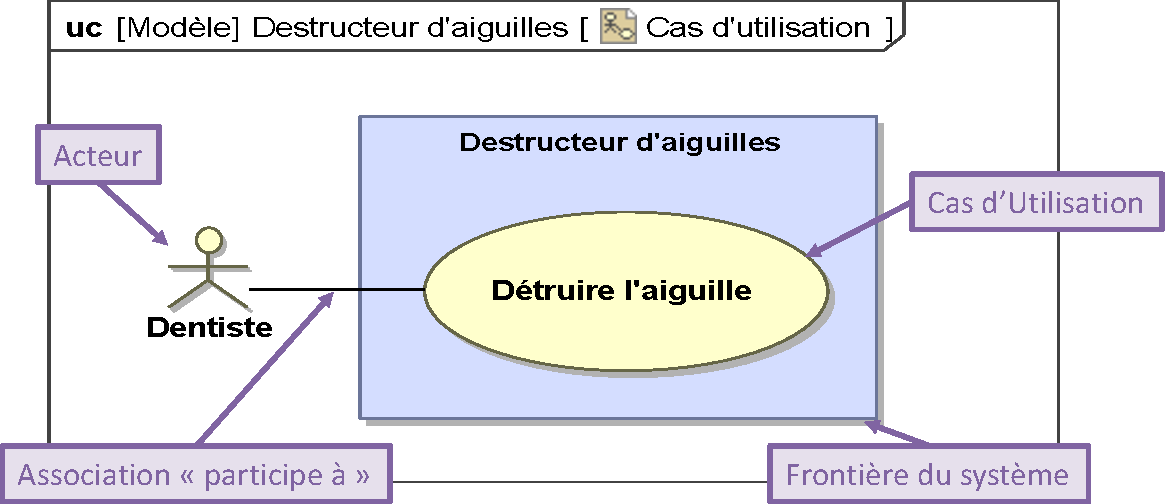
\includegraphics[width=\linewidth]{img/Use_case}
 \caption{Diagramme des Cas d'Utilisation}
\end{minipage}
 \hfill
\begin{minipage}{0.45\linewidth}

Il présente la frontière du système avec à l'intérieur les \textbf{cas d'utilisation} (verbe à l'infinitif à l'intérieur d'une bulle). Il peut en exister plusieurs mais souvent, un seul suffit. Autour se placent les acteurs (ils constatent les services rendus du système).

\end{minipage}
\end{figure}

\begin{minipage}{0.4\linewidth}
Chaque cas d'utilisation: 
\begin{itemize}
 \item possède un point de départ (élément déclenchant),
 \item suit une succession d'étapes,
 \item se termine (service rendu).
\end{itemize}
\end{minipage}
\hfill
\begin{minipage}{0.55\linewidth}
\begin{warn}
Il ne s'agit que des \textbf{fonctionnalités} pour lesquelles le système \textbf{a été prévu}, par exemple, une voiture n'existe pas pour être rechargée en carburant, c'est une exigence et pas une fonctionnalité.
\end{warn}
\end{minipage}
}}

{\frame{
\frametitle{Les messages pour un cas d'utilisation}
\begin{figure}[!h]
\begin{minipage}{0.4\linewidth}
 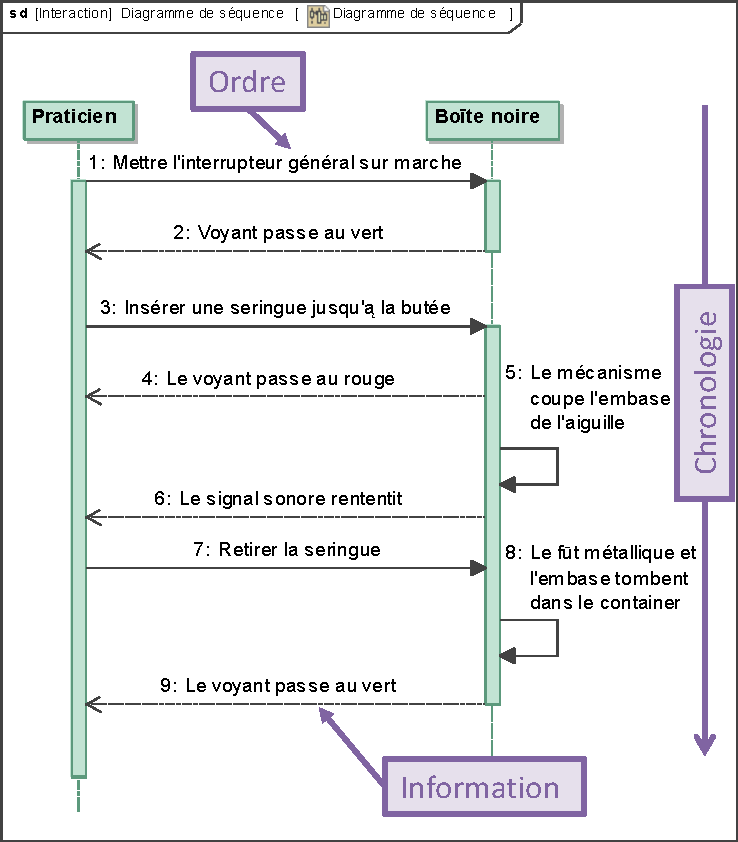
\includegraphics[width=\linewidth]{img/Sequence}
 \caption{Diagramme de Séquence}
\end{minipage}
 \hfill
\begin{minipage}{0.57\linewidth}
Un \textbf{cas d'utilisation} peut être vu comme un \textbf{scénario} durant lequel il existe une \textbf{interaction} (communication) entre un acteur et le système.Ils s'échangent des \textbf{ordres} ou des \textbf{informations}. Le \textbf{diagramme de séquence} permet de présenter cette interaction, il répond à la question : \og Comment est réalisé ce cas d'utilisation ? \fg.

\begin{itemize}
 \item Il existe au moins un diagramme de séquence pour chaque cas d'utilisation,
 \item Il montre les interactions entre différents éléments d'un point de vue séquentiel (ordre chronologique),
 \item Les messages peuvent être échangés entre l'acteur et le système mais aussi entre éléments du système.
\end{itemize}
\end{minipage}
\end{figure}
}}

{\frame{
\frametitle{Le retour aux exigences}
\begin{figure}[!h]
\begin{minipage}{0.3\linewidth}
 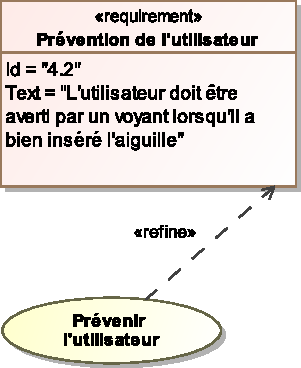
\includegraphics[width=\linewidth]{img/Use_case_2}
 \caption{Diagramme des Exigences}
\end{minipage}
 \hfill
\begin{minipage}{0.65\linewidth}
L'objectif étant la rédaction d'un \textbf{cahier des charges} et donc d'un \textbf{diagramme des exigences} le plus complet possible, il est nécessaire après avoir fait une étude des cas d'utilisation et des interactions associées d'\textbf{intégrer ces résultats} dans le diagramme des exigences afin de le faire évoluer.

\begin{itemize}
 \item Une fois complété, le diagramme des exigences devient un moyen de communication entre les participants à la conception,
 \item Il peut même être découpé en fonction des informations à donner à certains sous-traitants.
\end{itemize}
\end{minipage}
\end{figure}


}}

{\frame{
\frametitle{Il faut répondre au cahier des charges....}

\begin{savoir}

Vous devez être capables :
\begin{itemize}
 \item de prendre en compte le contexte d'un produit et les acteurs à qui il rend service,
 \item d'étudier les interactions qui interviennent dans chaque cas d'utilisation d'un produit.
\end{itemize}
\end{savoir}

\begin{prob}

L'objectif de la conception est la création ou l'adaptation d'un produit.
\begin{itemize}
 \item \textit{Problème: Comment trouver la solution qui répondra aux exigences ?}
 \item \textbf{Perspectives}: Trouver une méthode pour être sûr de toutes les prendre en compte et une seule fois.
\end{itemize}
\end{prob}
}}

\section{Les solutions techniques}

\ifdef{\prive}{}{
\begin{frame}
\frametitle{Table des matières}
\tableofcontents[currentsection]
\end{frame}}

{\frame{
\frametitle{Solutions techniques}

Le \textbf{cahier des charges} d'un produit consiste à définir l'ensemble des spécifications qui feront que le produit permette de rendre les \textbf{services attendus} pour tous ces cas d'utilisation.

\begin{itemize}
 \item L'étape suivante consiste à déterminer les \textbf{solutions techniques} à ces exigences,
 \item L'ensemble des solutions techniques constituera le \textbf{système réel}.
\end{itemize}


\begin{minipage}{0.75\linewidth}
\begin{exemple}
\begin{itemize}
 \item Une solution technique peut répondre à plusieurs exigences,
 \item Le plus souvent elle est dédié à une exigence.
\end{itemize}
\end{exemple}
\end{minipage}
\hfill
\begin{minipage}{0.2\linewidth}
  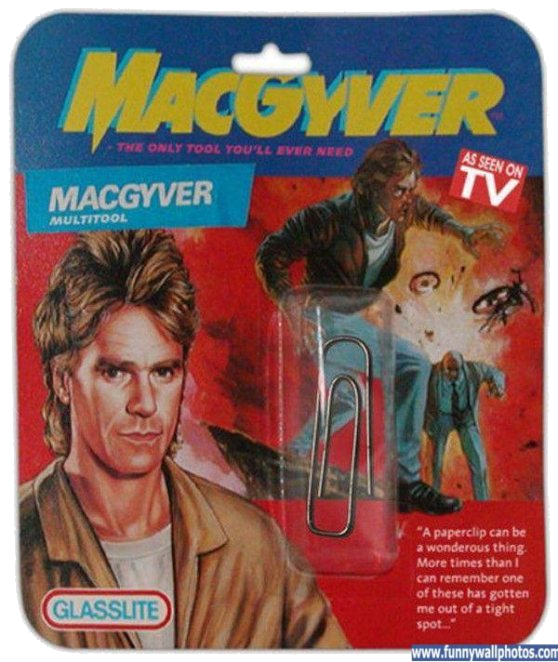
\includegraphics[width=0.9\linewidth]{img/mac_gyver}
\end{minipage}

\vfill

Il est très important d'avoir une bonne \textbf{culture technologique} afin d'avoir une base de \textbf{solutions technologiques} sur laquelle s'appuyer lorsqu'on cherche une solution à un problème.

Il existe des \textbf{bases de données} de solutions techniques, basées sur des \textbf{brevets}, qui permettent de compléter cette culture (Méthode TRIZ).
}}

{\frame{
\frametitle{Association de solutions techniques à des exigences}

Il est très important lors d'une conception de capitaliser un maximum d'information et notamment les choix de solutions qui ont été faits. 

\begin{minipage}{0.4\linewidth}
Cela a les avantages suivants :
\begin{itemize}
 \item Si une exigence apparaît plusieurs fois (ou dans une autre conception) de réutiliser cette solution,
 \item Si une exigence disparaît (reconception) la solution technique peut alors être retirée du système.
\end{itemize}
La solution technique est présentée sous la forme d'un \textbf{bloc} (décrit plus tard).
\end{minipage}
\hfill
\begin{minipage}{0.55\linewidth}
  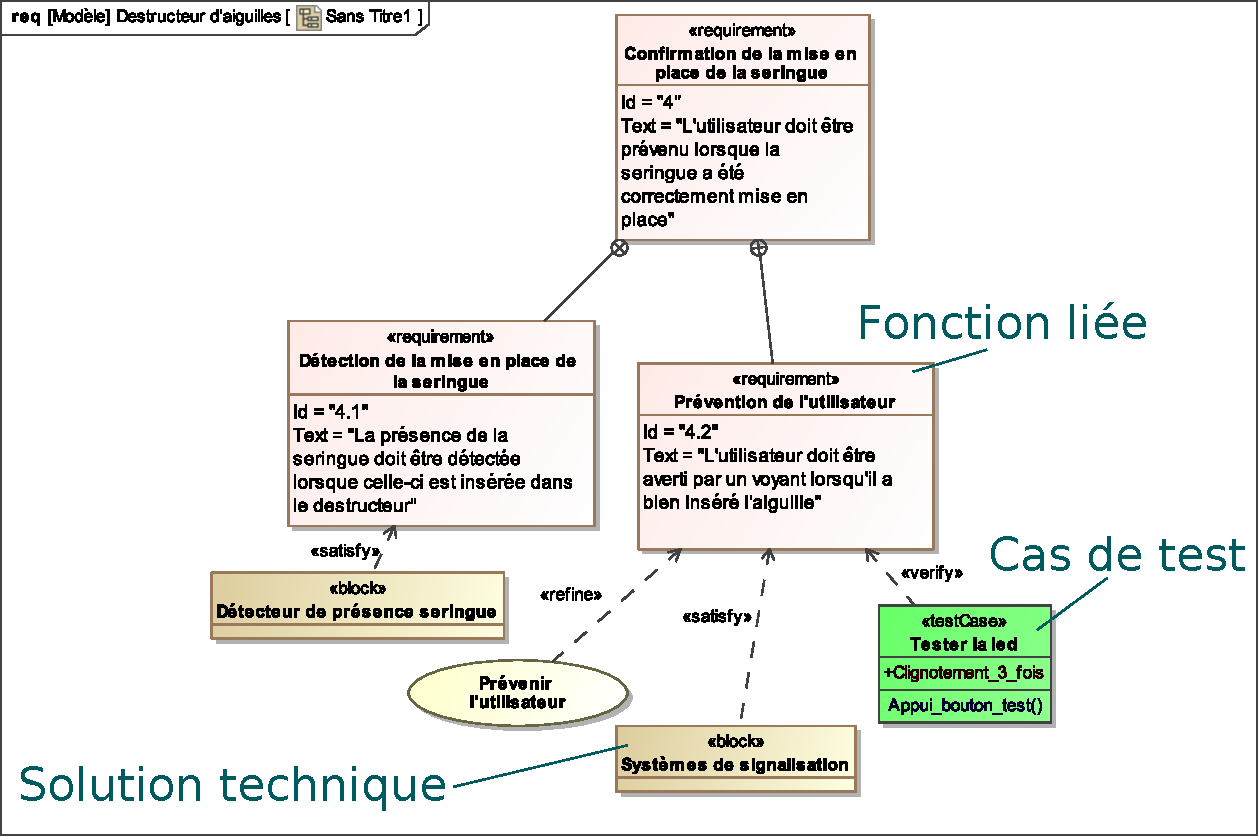
\includegraphics[width=0.9\linewidth]{img/Bloc7}
\end{minipage}

\vfill

L'\textbf{association} de solutions techniques à une exigence se fait directement dans le \textbf{diagramme d'exigence} grâce à la fonction \og satisfy \fg.
}}

{\frame{
\frametitle{Que faire des solutions techniques...}

\begin{savoir}
Vous devez être capables :
\begin{itemize}
 \item d'analyser pour qu'elle exigence une solution technique a été intégrée à un système,
 \item de déterminer quelle solution technique répond à un exigence.
\end{itemize}
\end{savoir}

\begin{prob}

Un système est un ensemble \textbf{organisé} de solutions techniques.
\begin{itemize}
 \item \textit{Problème: Comment représenter cette organisation ?}
 \item \textbf{Perspectives}: Trouver un moyen de relier les différentes solutions techniques et de caractériser ces liens.
\end{itemize}
\end{prob}
}}

\section{Décomposition structurelle}

\ifdef{\prive}{}{
\begin{frame}
\frametitle{Table des matières}
\tableofcontents[currentsection]
\end{frame}}

{\frame{
\frametitle{Le structure du système}

\begin{minipage}{0.3\linewidth}
  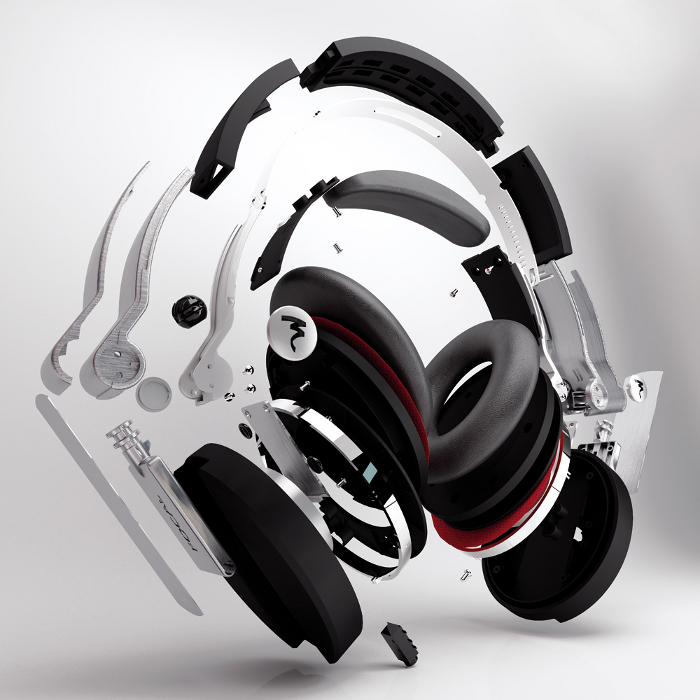
\includegraphics[width=0.9\linewidth]{img/casque}
\end{minipage}
\hfill
\begin{minipage}{0.65\linewidth}
Un \textbf{système} est constitué de plusieurs \textbf{solutions techniques} (sous-systèmes, pièces,...). Les liens qui existent entre ces solutions techniques constitue la \textbf{structure} du système. Ces liens peuvent être de plusieurs sortes:
\begin{itemize}
 \item assemblage mécanique,
 \item transfert d'énergie,
 \item échange d'information.
\end{itemize}
\end{minipage}

\begin{minipage}{0.8\linewidth}
Afin de représenter la structure d'un système, il existe différentes solutions:
\begin{itemize}
 \item le \textbf{diagramme de définition de bloc (BDD):} Sur ce diagramme chaque composant (sous-système, composant, élément externe,...) est représenté par un \textbf{bloc} qui intégrera toutes les données nécessaires à sa caractérisation,
 \item les \textbf{chaînes d'information et d'énergie:} Ce diagramme présente les fonctions classiques qui caractérisent un système complexe.
\end{itemize}

\end{minipage}
\hfill
\begin{minipage}{0.15\linewidth}

  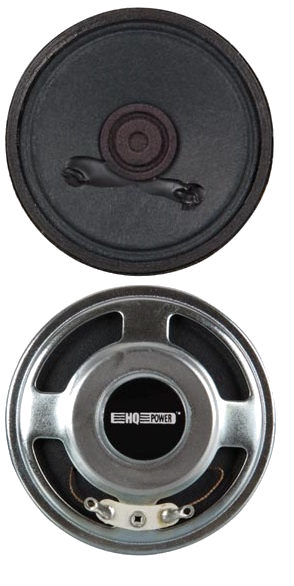
\includegraphics[width=0.9\linewidth]{img/hp}
\end{minipage}
}}

{\frame{
\frametitle{La représentation par blocs}

\begin{minipage}{0.6\linewidth}
Un bloc peut être un acteur, un élément externe ou un composant du système. Il est caractérisé par quelques éléments:
\begin{itemize}
 \item ses propres composants,
 \item les éléments avec lesquels il interagit,
 \item des ports (connexions avec l'extérieur) via lesquels transitent des flux.
\end{itemize}
\end{minipage}
\hfill
\begin{minipage}{0.35\linewidth}
  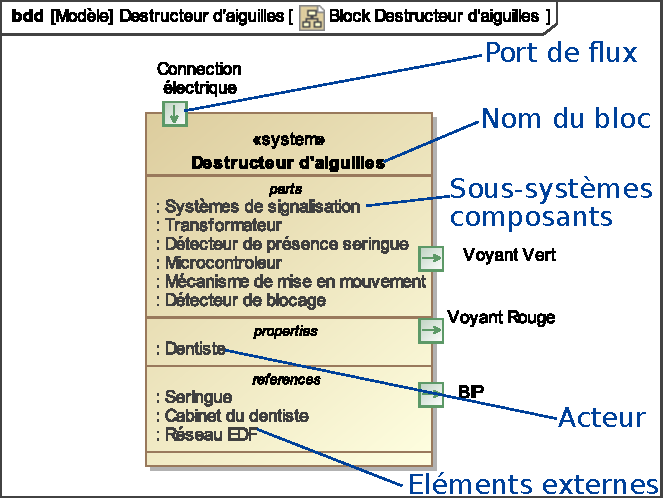
\includegraphics[width=0.9\linewidth]{img/Bloc1}
\end{minipage}

\vfill

\begin{figure}[!h]
\begin{minipage}{0.2\linewidth}
 \centering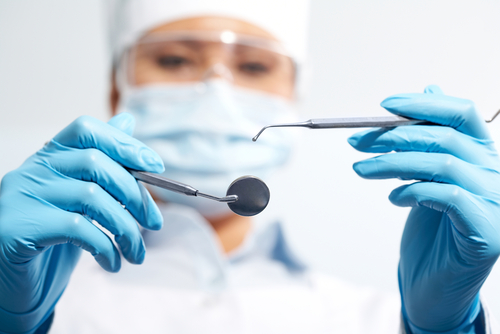
\includegraphics[height=1.5cm]{img/dentiste}
 \caption{Dentiste}
\end{minipage}
\hfill
\begin{minipage}{0.23\linewidth}
 \centering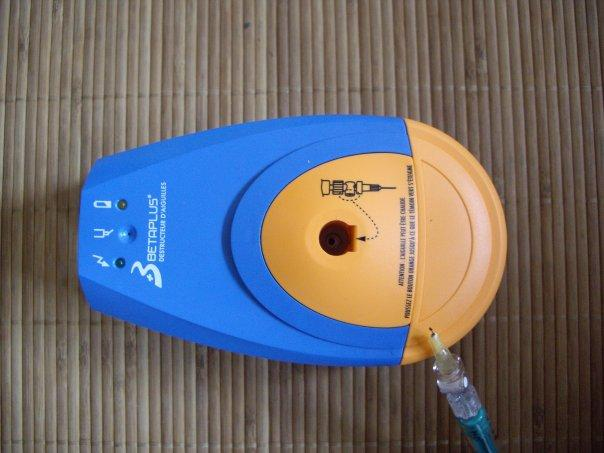
\includegraphics[height=1.5cm]{img/destructeur}
 \caption{Destructeur}
 \end{minipage}
\hfill
\begin{minipage}{0.23\linewidth}
 \centering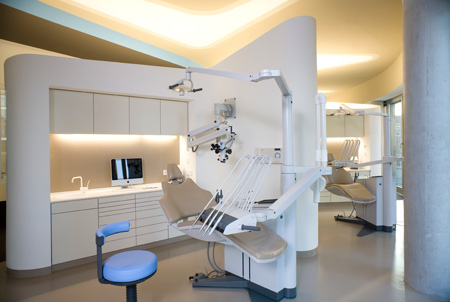
\includegraphics[height=1.5cm]{img/cabinet}
 \caption{Cabinet}
\end{minipage}
\hfill
\begin{minipage}{0.23\linewidth}
 \centering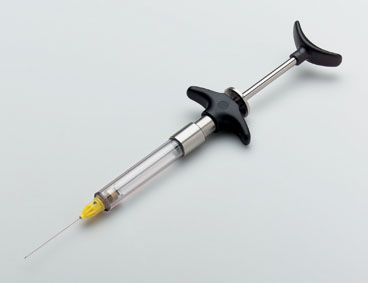
\includegraphics[height=1.5cm]{img/seringue}
 \caption{Seringue}
\end{minipage}
\end{figure}

Ces blocs sont reliés entre eux dans un \textbf{diagramme de blocs}.

}}

{\frame{
\frametitle{L'architecture des blocs}

\begin{minipage}{0.45\linewidth}
\textbf{Composition:}

La relation de composition existe lorsqu'un bloc englobe ses parties, le côté du tout indiqué par un losange plein.

\centering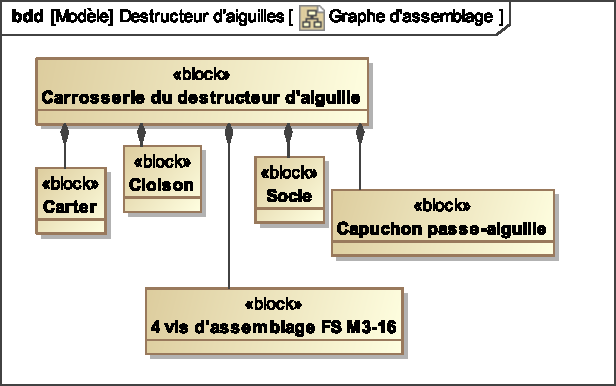
\includegraphics[width=0.6\linewidth]{img/Bloc3}
\end{minipage}
\hfill
\begin{minipage}{0.45\linewidth}
\textbf{Agrégation:}

Similaire à la composition, cependant, les parties ne sont pas nécessaires au tout, le côté du tout indiqué par un losange blanc.

\centering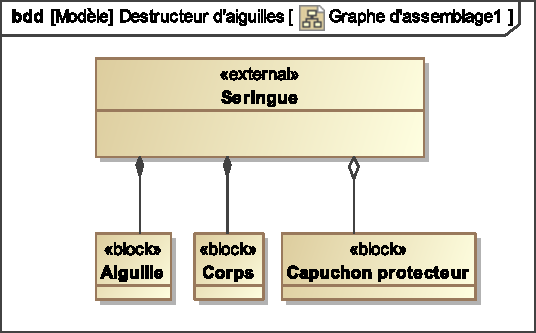
\includegraphics[width=0.6\linewidth]{img/Bloc2}
\end{minipage}

\vfill

\begin{minipage}{0.5\linewidth}
\textbf{Généralisation:}

Il est possible de factoriser des propriétés communes (valeurs, parties, etc.) ainsi des blocs  \og héritent \fg des propriétés du bloc généralisé.

\end{minipage}
\hfill
\begin{minipage}{0.4\linewidth}
\centering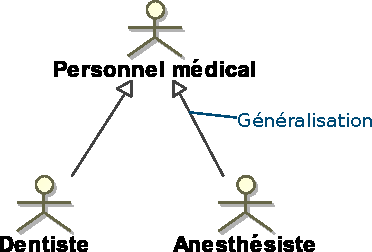
\includegraphics[width=0.7\linewidth]{img/Bloc4}
\end{minipage}
}}

{\frame{
\frametitle{Les échanges entre les blocs}

L'étape suivante consiste a étudier les \textbf{flux} qui circulent entre les sous-composants d'un système. Pour cela, chaque élément peut être \textbf{décomposé} en sous-composants qui apparaissent dans un \textbf{diagramme de blocs interne}.

\vspace{-0.5cm}

\begin{center}
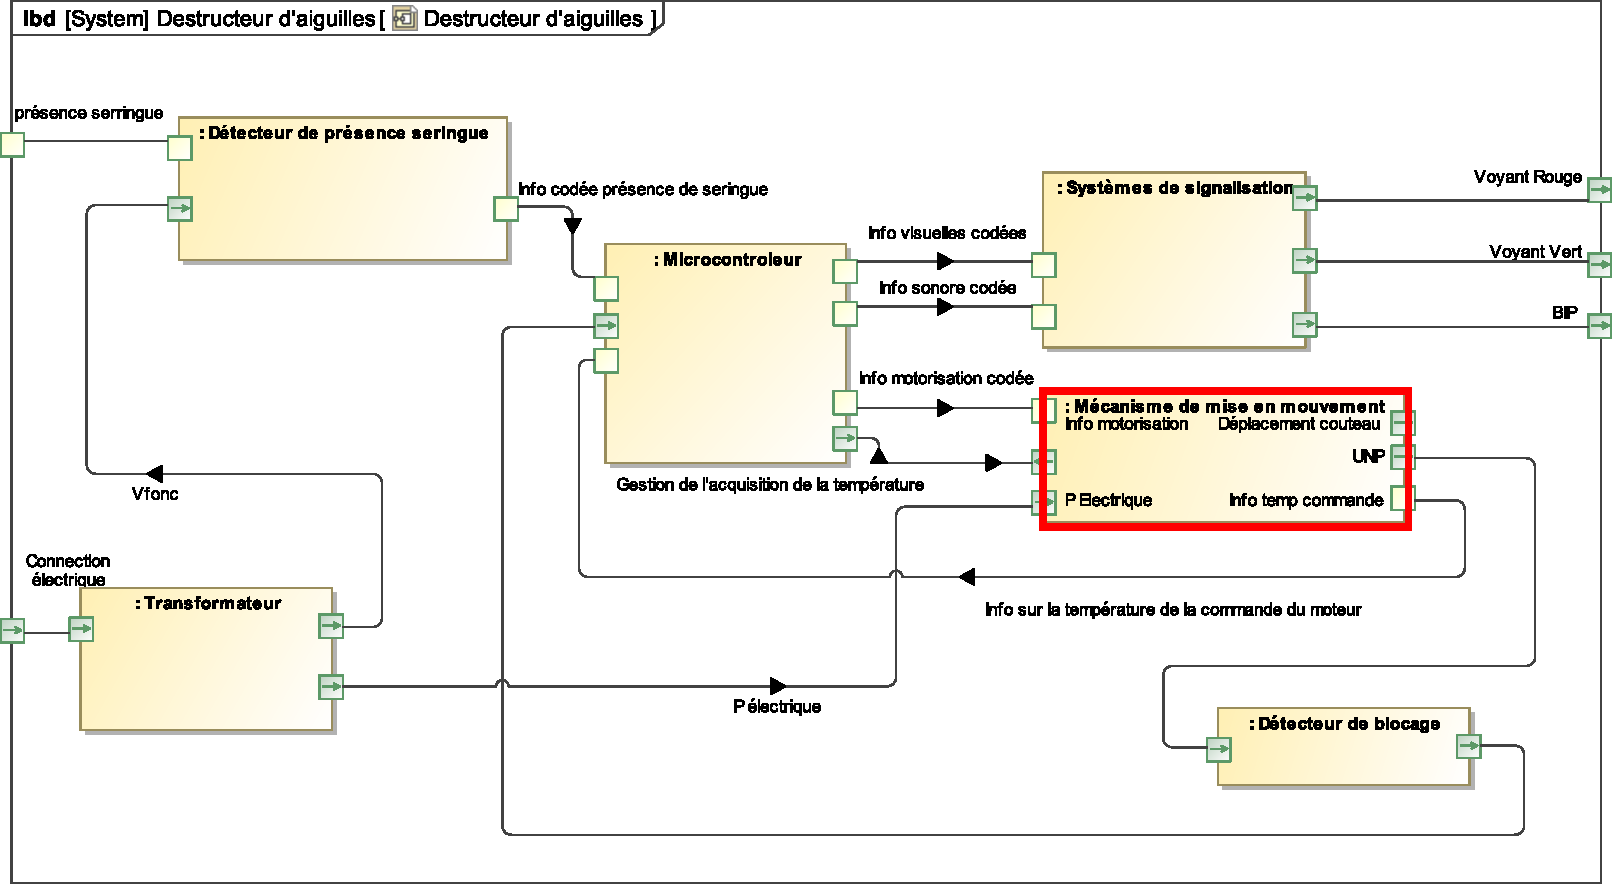
\includegraphics[width=0.8\linewidth]{img/IBD1}
\end{center}

\vspace{-0.5cm}

Des flux circulent entre ces composants et \textbf{interagissent} avec les composants par l'intermédiaire de \textbf{ports}.
}}

{\frame{
\frametitle{Description du sous-système}

Le diagramme suivant présente le diagramme des blocs interne du \textit{mécanisme de mise en mouvement}.

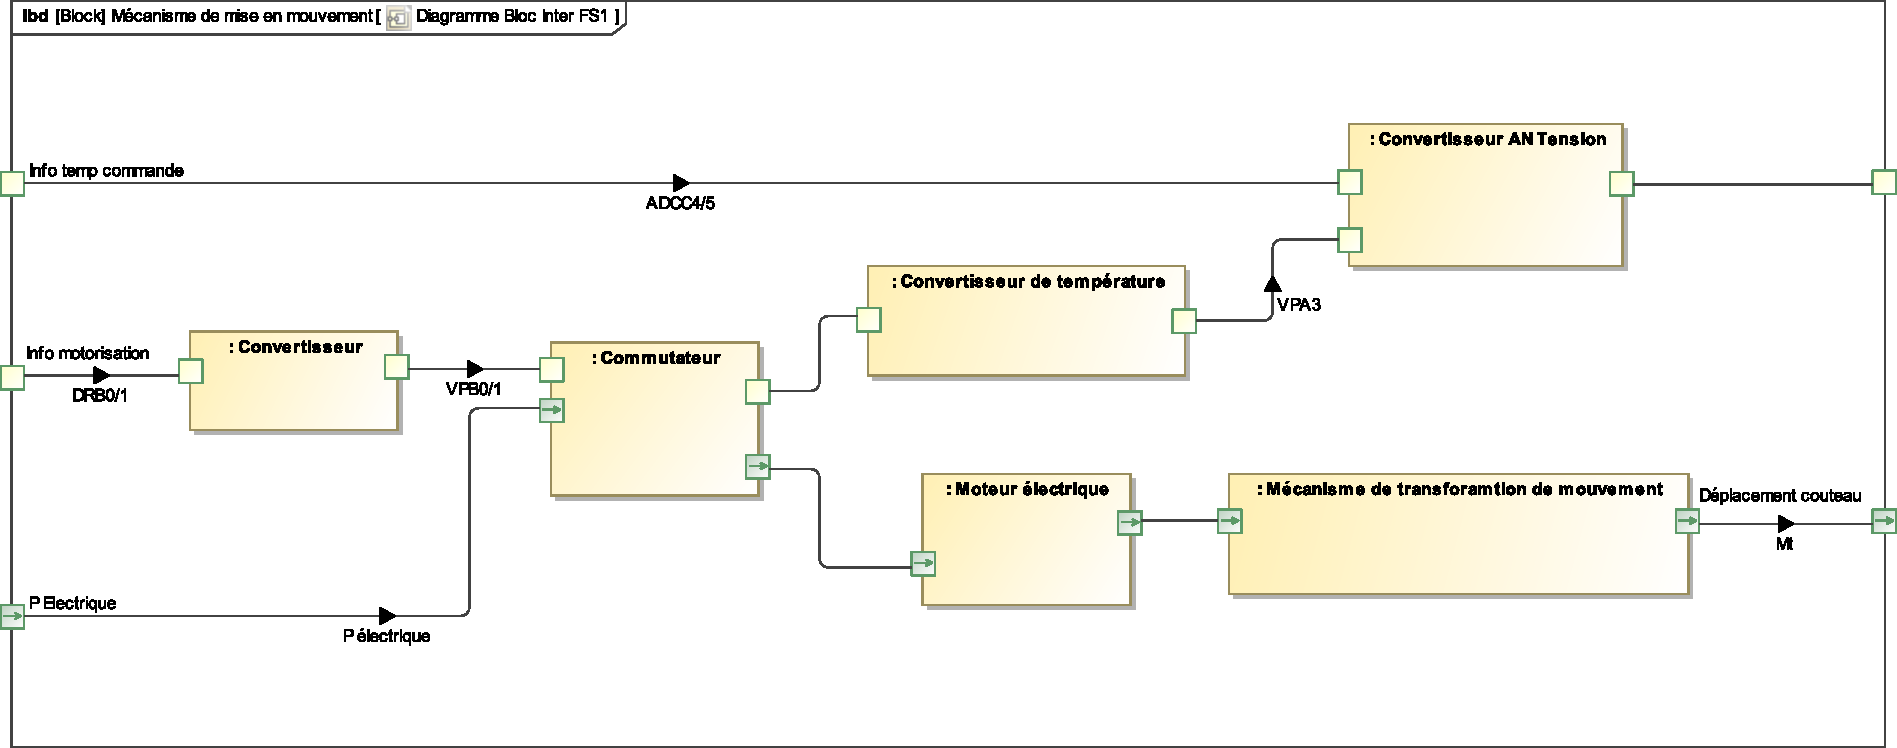
\includegraphics[width=\linewidth]{img/IBD2}

Les ports du bloc précédent correspondent à ceux de la nouvelle frontière d'étude.
}}

{\frame{
\frametitle{Des ports et des flux}

La connexion entre un flux et un bloc est représentée par un \textbf{port}. Les ports définissent les points d'\textbf{interaction} entre les blocs. Il peuvent être de deux natures:
\begin{itemize}
 \item \textbf{flux (flow port):} ce type de port autorise la circulation de flux physiques entre les blocs,
 \item \textbf{standard:} ce type de port autorise la description de services logiques entre les blocs.
\end{itemize}

\centering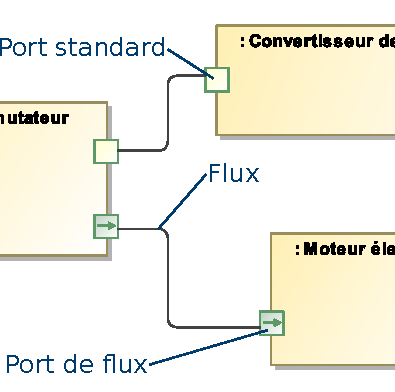
\includegraphics[width=0.4\linewidth]{img/IBD3}

}}

{\frame{
\frametitle{Un système et son architecture}

\begin{savoir}
Vous devez être capables :
\begin{itemize}
 \item de décrire l'architecture d'un système,
 \item de hiérarchiser ses composants,
 \item de caractériser les flux qui le traverse.
\end{itemize}
\end{savoir}

\begin{prob}

Il est nécessaire d'utiliser d'autres formes de représentation d'un mécanisme.
\begin{itemize}
 \item \textit{Problème: Comment représenter la géométrie d'un mécanisme ?}
 \item \textbf{Perspectives}: Trouver un modèle de description d'un mécanisme adapté aux situations pour lesquelles le langage SysMl n'est pas prévu.
\end{itemize}
\end{prob}


}}

\end{document}

